\documentclass[a4paper,11pt]{jsarticle}


% 数式
\usepackage{amsmath,amsfonts}
\usepackage{bm}
\usepackage{url}
% 画像
\usepackage[dvipdfmx]{graphicx}
\usepackage[dvipdfmx]{color}
\usepackage{here} % 図を指定した位置に強制的に配置するためのパッケージ
\usepackage{amsmath} %数学記号を拡充するパッケージ
\usepackage{multirow}
\renewcommand{\labelenumi}{(\arabic{enumi}).}
\renewcommand\thefootnote{注 \arabic{footnote}} % 脚注の番号表記をロマン数字に設定するためのおまじない
\usepackage[dvipdfmx]{hyperref}
\usepackage{pxjahyper}
\usepackage{dcolumn}
\usepackage{longtable}
\usepackage[hang,small,bf]{caption}
\usepackage[subrefformat=parens]{subcaption}
\newcolumntype{d}[1]{D{.}{.}{#1}}
\newcommand{\ctext}[1]{\raise0.2ex\hbox{\textcircled{\scriptsize{#1}}}}
\hypersetup{% hyperrefオプションリスト
setpagesize=false
bookmarksnumbered=true,%
bookmarksopen=true,%
colorlinks=true,%
linkcolor=blue,
citecolor=red,
urlcolor=blue,
}

\title{}
\date{\today}
\author{\\
学籍番号:1111\\
氏名:桃太郎}

\begin{document}
\maketitle

\newpage

\section{目的}
\section{原理}
\section{方法}
\section{結果}
\section{考察}
\section{結論}

%画像

\begin{figure}[H]
  \centering
  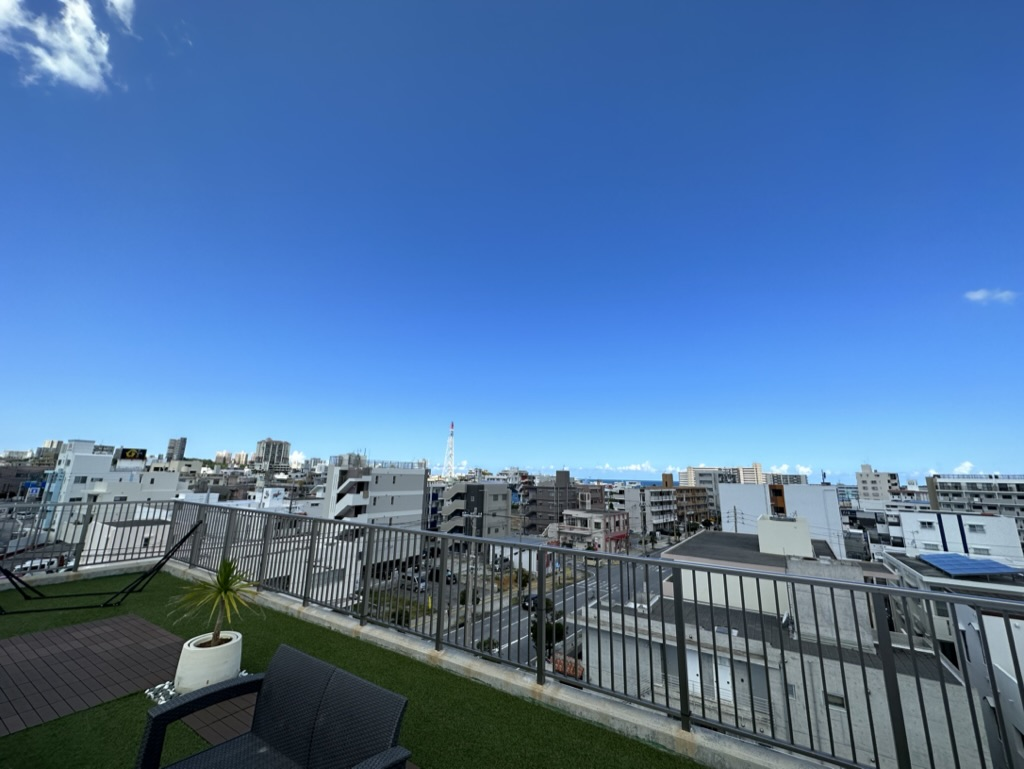
\includegraphics[width=14cm]{Introduce.jpeg}
  \caption{キャプション} 
\end{figure}


%表
\begin{table}[H]
  \begin{center}
  \caption{キャプション}
  \begin{tabular}{cc} \hline
  1 &   2 \\ \hline
  0   & 0  \\
  45  & 30  \\
  90  & 60  \\
  135 & 90  \\
  180 & 120  \\
  \hline
\end{tabular}
\end{center}
\end{table}

\begin{thebibliography}{99}
  \bibitem{a}  参考文献
\end{thebibliography}
  
\end{document}